% ****** Start of file aipsamp.tex ******
%
%   This file is part of the AIP files in the AIP distribution for REVTeX 4.
%   Version 4.1 of REVTeX, October 2009
%
%   Copyright (c) 2009 American Institute of Physics.
%
%   See the AIP README file for restrictions and more information.
%
% TeX'ing this file requires that you have AMS-LaTeX 2.0 installed
% as well as the rest of the prerequisites for REVTeX 4.1
% 
% It also requires running BibTeX. The commands are as follows:
%
%  1)  latex  aipsamp
%  2)  bibtex aipsamp
%  3)  latex  aipsamp
%  4)  latex  aipsamp
%
% Use this file as a source of example code for your aip document.
% Use the file aiptemplate.tex as a template for your document.
\documentclass[%
 aip,
% jmp,
% bmf,
% sd,
% rsi,
 amsmath,amssymb,
%preprint,%
 reprint,%
%author-year,%
%author-numerical,%
% Conference Proceedings
]{revtex4-1}

\usepackage{graphicx}% Include figure files
\usepackage{dcolumn}% Align table columns on decimal point
\usepackage{bm}% bold math
\usepackage{verbatim}
%\usepackage[mathlines]{lineno}% Enable numbering of text and display math
%\linenumbers\relax % Commence numbering lines

\usepackage[utf8]{inputenc}
\usepackage[T1]{fontenc}
\usepackage{mathptmx}
\usepackage{etoolbox}

%% Apr 2021: AIP requests that the corresponding 
%% email to be moved after the affiliations
\makeatletter
\def\@email#1#2{%
 \endgroup
 \patchcmd{\titleblock@produce}
  {\frontmatter@RRAPformat}
  {\frontmatter@RRAPformat{\produce@RRAP{*#1\href{mailto:#2}{#2}}}\frontmatter@RRAPformat}
  {}{}
}%
\makeatother
\begin{document}

\preprint{AIP/123-QED}

\title[Intermediate Physics Laboratory 2, Module 1]{Measuring DUT resistance and capacitance in parallel circuits connected to an AC voltage}
% Force line breaks with \\
\author{Myeong-gi Jo}
\altaffiliation{
whaudrl4005@gmail.com
}
\author{Subin Kim}
\altaffiliation{
subini0213@snu.ac.kr
}
\author{Jeong Min Lee}
\altaffiliation{
jmleeluck@snu.ac.kr
}
\author{Eugene Park}
\altaffiliation{
eupark@snu.ac.kr
}
\affiliation{ 
Department of Physics and Astronomy, Seoul National University
}



\date{\today}
\begin{abstract}
In the realm of electrical experiments, accurate knowledge of electrical component parameters is fundamental. This study presents an exploration of error analysis applied to a simple passive component system comprising resistors and capacitors. The objective is to measure resistance and capacitance for each resistor and capacitor as devices under test (DUTs). Despite the simplicity of passive components, we report an anomalous frequency response of the resistor and possible intrinsic fluctuations in the capacitance measured. This research also categorizes errors encountered at various frequencies into two groups: systematic and statistical. The origins of these errors are discussed, and conditions for achieving precision in electrical measurements are established. This work contributes valuable insights into the assessment and mitigation of errors in electrical experimentation, providing a foundation for more accurate and reliable results in future studies.

\end{abstract}

\maketitle

\section{\label{sec:Intro} Introduction} 

For every electrical experiment, knowing the parameters and features of the electrical components is essential. The precise value of them can be obtained by proper error analysis. Through error analysis methods, a firm understanding of the bounds an experiment can reveal is established. We divide error into two classifications: \textit{statistical error} and \textit{systematic error}. Statistical error originates from random fluctuations intrinsic in any physical value. Systematic error in this context refers to an error that is caused by limitations of the system, for instance, measurement resolutions. Thus, in planning an experiment, an important part is to construct an estimation of the quantity of error that would be present. Such information supports whether the experiment is sufficient to claim its findings. 

In this experiment, we implement this process to a simple passive component system consisting of resistors and capacitors in parallel. To estimate the $R_{\textrm{DUT}}$ and $C_{\textrm{DUT}}$ in this system, we measured the voltage amplitude ratios($r_V$) and phase differences($\phi$) under a sinusoidal voltage input to evaluate the impedance of a resistor-capacitor. The main formulae to find the $R_{\textrm{DUT}}$ and $C_{\textrm{DUT}}$ are the following. (Derivation of following equations can be found in \textbf{\textsf{Appendix A}}.)
\begin{comment}
    parallel series component. (Derivation of following equations can be found in \textbf{Appendix A}.)
\end{comment}


\begin{equation}
Z=\frac{(R_{\textrm{ref}}+R_{\textrm{DUT}})+i\omega R_{\textrm{ref}} C_{\textrm{DUT}}R_{\textrm{DUT}}}{1+i\omega C_{\textrm{DUT}}R_{\textrm{DUT}}}
\end{equation}

\begin{equation}
r_{V}=R_{\textrm{ref}}\sqrt{\frac{1+\omega^{2}C_{\textrm{DUT}}^{2}R_{\textrm{DUT}}^{2}}{(R_{\textrm{ref}}+R_{\textrm{DUT}})^{2}+\omega^{2}R_{\textrm{ref}}^{2}C_{\textrm{DUT}}^{2}R_{\textrm{DUT}}^{2}}}
\end{equation}

\begin{equation}
\phi=\tan^{-1}\frac{-\omega C_{\textrm{DUT}}R_{\textrm{DUT}}^{2}}{R_{\textrm{ref}}+R_{\textrm{DUT}}+\omega^{2} R_{\textrm{ref}}C_{\textrm{DUT}}^{2}R_{\textrm{DUT}}^{2}}
\end{equation}

\noindent These values are further extended to measure the resistor and capacitor, each being a device under testing(DUT). The frequency response of each DUT is also analyzed.

Extending the analysis, the experimental error by different frequencies is also divided into systematic error and statistical error. We then explain the dominant origins of both errors and establish conditions for precision measurement of the current system. Such analysis can be extended to more complicated systems to provide measures for estimating the error. 

The manuscript is organized as follows. First, in Methods we elaborate the experimental procedure and the theoretical calculations for partial derivatives. Means of error propagation and error analysis are also discussed. The DUT value distributions, measurement results, and error analysis are shown in \textbf{\textsf{Results}}. Discussion holds implications of the results, mainly on explaining the frequency response of DUT components and their error. 

\section{\label{sec:Methods} Methods}
\subsection{Experimentation}
The circuit schematic is shown in Fig. \ref{fig:basic}(a). The measured voltages are $V_{\textrm{total}}$, $V_{R_{\textrm{ref}}}$, and a sinusoidal voltage source is given via $V_0$. The resistor and capacitor measured are $R_{\textrm{DUT}}$ and $C_{\textrm{DUT}}$. $R_{\textrm{ref}}$ is the reference resistor which is known \textit{a priori}. The circuit was assembled on a breadboard, and all used resistor values were measured with a multimeter Fluke 87.

We performed the experiment with the waveform generator($V_0$) and voltage inputs($V_{\textrm{total}}$, $V_{R_{\textrm{ref}}}$) of Analog Discovery 2(AD2). The waveform generator was set to give a sinusoidal wave of amplitude $2.5$V for frequencies $100$Hz to $2000$Hz in $20$Hz steps. The measuring time was set to $100$ periods, and the first and last period was discarded to avoid intrinsic effects. This ensures coherent sampling. Each frequency step was repeated $100$ times. An addition of $5000$ repetitions at $1000$Hz were conducted. The total procedure was repeated for three different reference resistors $R_{\textrm{ref}} = 4.7\text{k}\Omega, 7.5\text{k}\Omega, 12.2\text{k} \Omega$.

An identical set of measurements was performed as a comparison group without the resistor-capacitor parallel component in place and instead shorted with a conducting wire. These control experiment values were used to compensate for external circuit effects other than the DUT components. 

The input/output rate was set to $100$kHz, and the voltage input ranges were set to $-2.5$V to $2.5$V for all measurements.

\subsection{DUT Value Theoretical Calculation}
 From the impedance (1), we calculated the voltage amplitude ratio and phase difference between the reference resistor and waveform input as (2) and (3) respectively. Substituting the measured value of $R_{\textrm{ref}}$, $\omega$, $r_{V}$, $\phi$ in (2) and (3), we can obtain $R_{\textrm{DUT}}$ and $C_{\textrm{DUT}}$ through MATLAB.

\subsection{Partial Derivative of DUT Values}

In this experiment, the error of $R_{\textrm{DUT}}$ and $C_{\textrm{DUT}}$ is affected by the partial derivatives with respect to $r_{V}$, $\phi$, $\omega$, $R_{\textrm{ref}}$. If the absolute value of the derivative is large, the error is prone to be large, and vice versa.  Instead of solving (2) and (3) for $R_{\textrm{DUT}}$ and $C_{\textrm{DUT}}$ explicitly, we can get desired derivatives more easily by solving linear equations. By doing so, we obtain the desired partial derivatives.
\begin{align}
&\frac{\partial R_{\textrm{DUT}}}{\partial r_{V}}=-\frac{\frac{\partial \phi}{\partial C_{\textrm{DUT}}}}{\frac{\partial \phi}{\partial R_{\textrm{DUT}}}\frac{\partial r_{V}}{\partial C_{\textrm{DUT}}} - \frac{\partial r_{V}}{\partial R_{\textrm{DUT}}}\frac{\partial \phi}{\partial C_{\textrm{DUT}}}}\\
&\frac{\partial R_{\textrm{DUT}}}{\partial \phi}=\frac{\frac{\partial r_{V}}{\partial C_{\textrm{DUT}}}}{\frac{\partial \phi}{\partial R_{\textrm{DUT}}}\frac{\partial r_{V}}{\partial C_{\textrm{DUT}}} - \frac{\partial r_{V}}{\partial R_{\textrm{DUT}}}\frac{\partial \phi}{\partial C_{\textrm{DUT}}}}
\end{align}

\begin{align}
&\frac{\partial C_{\textrm{DUT}}}{\partial r_{V}}=\frac{\frac{\partial \phi}{\partial R_{\textrm{DUT}}}}{\frac{\partial \phi}{\partial R_{\textrm{DUT}}}\frac{\partial r_{V}}{\partial C_{\textrm{DUT}}} - \frac{\partial r_{V}}{\partial R_{\textrm{DUT}}}\frac{\partial \phi}{\partial C_{\textrm{DUT}}}}\\
&\frac{\partial C_{\textrm{DUT}}}{\partial \phi}=-\frac{\frac{\partial r_{V}}{\partial R_{\textrm{DUT}}}}{\frac{\partial \phi}{\partial R_{\textrm{DUT}}}\frac{\partial r_{V}}{\partial C_{\textrm{DUT}}} - \frac{\partial r_{V}}{\partial R_{\textrm{DUT}}}\frac{\partial \phi}{\partial C_{\textrm{DUT}}}}
\end{align}


\subsection{Measurements and Corresponding Error}
\subsubsection{Reference Resistors}
A total of three reference resistors with labeled resistances $4.7\text{k}\Omega$, $7.5\text{k}\Omega$, $12.2\text{k}\Omega$ were selected. For accurate experimentation, the resistance was measured with a Fluke 87 multimeter, and the systematic error of the measurements was referred from the datasheet\cite{multimeter}. Thus, we obtained $4.673\pm0.006\text{k}\,\Omega$, $7.44\pm0.015\text{k}\,\Omega$, $12.11\pm0.016\text{k}\,\Omega$. 
The DUT resistor value $99.7\pm0.15\text{k}\Omega$ was also measured with the same device for comparison.

\subsubsection{Voltage Amplitude Ratio}
The voltage amplitude of both signals was obtained by calculating the root-mean-square(RMS) of the analog input signal. Since waveform generates an accurate sinusoidal wave, the RMS of the signal is the voltage amplitude times a factor of $1/\sqrt{2}$.

The specified absolute resolution of the AD2 analog input is $0.32$mV when the scale is less than $0.5$V/div\cite{ad2spec}. This was used to calculate the systematic error of the voltage amplitude ratio. The propagated systematic error of $r_{V}$ is then $\sigma_{r_{V}, \textrm{sys}}=(1.6\times10^{-4})(V_{R_{\textrm{ref}}}/V_{\textrm{total}})\>\sqrt{(1/V_{R_{\textrm{ref}}})^2 + (1/V_{\textrm{total}})^2}$.

\subsubsection{Frequency}
To confirm the frequency of the voltage signals generated from AD2, we performed the Fast Fourier Transform(FFT) to obtain the peak frequency. A rectangle sampling window was used.

The uncertainty of the FFT procedure is known as the following \cite{errorDFT}. 
\begin{equation}
    \sigma_{\textrm{FFT}} = \frac{\sigma_x}{\sqrt{N/2}}
    \label{eqn:errorDFT}
\end{equation}
where $x$ is the time sequence and $N$ is its length.

\subsubsection{Phase Difference}
For the measurement of the phase difference between $V_{R_{\textrm{ref}}}$ and $V_{\textrm{total}}$(Fig. \ref{fig:basic}(b)), we utilized the argument of the maximum FFT spectrum\cite{phaseDetection}. Furthermore, to perform proper statistical methods in $2\pi$ modular space, \textit{circular statistics} was implemented \cite{circStat}.

The uncertainty of the phase difference for a coherent rectangle sampling window propagates as follows\cite{phaseDetection}.
\begin{comment}
    \begin{align*}
        {\partial \phi \over \partial R} & = - \frac{I}{\left| \mathfrak{F}(x) \right|^2}, \quad {\partial \phi \over \partial I}  =  \frac{R}{\left| \mathfrak{F}(x) \right|^2} \\
        \therefore \sigma_{\phi}^2 = \left({\partial \phi \over \partial R}\right)^2\sigma_R^2 &+ \left({\partial \phi \over \partial I}\right)^2 \sigma_I^2 = \sigma_{DFT}^2 \frac{I^2 + R^2}{\left| \mathfrak{F}(x) \right|^4} = \frac{\sigma_{DFT}^2}{\left| \mathfrak{F}(x) \right|^2}
    \end{align*}
\end{comment}
\begin{equation}
    \sigma_{\phi}  = \frac{\sigma_{\textrm{DFT}}}{\left| \mathfrak{F}(x) \right|}
\end{equation}
\noindent where $\mathfrak{F}(x)$ is the FFT of target signal $x$ and $\sigma_{*}$ denotes the standard deviation of the parameter $*$.

\subsubsection{Systematic Error and Statistical Error}

From the error analysis above, we know systematic errors of voltage ratio($\sigma_{r_V}$), frequency($\sigma_{\omega}$), phase difference($\sigma_{\phi}$) and reference resistance($\sigma_{R_{\textrm{ref}}}$). Through equation (\ref{eq:rdut}) and (\ref{eq:cdut}), the propagated systematic error of a single measurement results in the following.

\begin{equation}
\sigma_{R_{\textrm{DUT,sys}}} = \sqrt{
    \begin{aligned}
    \left({\partial R_{\textrm{DUT}} \over \partial r_V}\sigma_{r_V}\right)^2&+\left({\partial R_{\textrm{DUT}} \over \partial \phi}\sigma_{\phi}\right)^2+\\
    &\left({\partial R_{\textrm{DUT}} \over \partial R_{\textrm{ref}}}\sigma_{R_{\textrm{ref}}}\right)^2+\left({\partial R_{\textrm{DUT}} \over \partial \omega}\sigma_{\omega}\right)^2
    \end{aligned}
    }\label{eqn:rduterror}
    \end{equation}
\begin{equation}
    \sigma_{C_{\textrm{DUT,sys}}} = \sqrt{
    \begin{aligned}
    \left({\partial C_{\textrm{DUT}} \over \partial r_V}\sigma_{r_V}\right)^2&+\left({\partial C_{\textrm{DUT}} \over \partial \phi}\sigma_{\phi}\right)^2+\\
    &\left({\partial C_{\textrm{DUT}} \over \partial R_{\textrm{ref}}}\sigma_{R_{\textrm{ref}}}\right)^2+\left({\partial C_{\textrm{DUT}} \over \partial \omega}\sigma_{\omega}\right)^2
    \end{aligned}
    }\label{cduterror}
\end{equation}

\noindent where $\sigma_{r_V}$, $\sigma_{\phi}$, $\sigma_{R_{\textrm{Ref}}}$, $\sigma_{\omega}$ are systematic errors of each.

From each repeated measurement of $R_{DUT}$ and $C_{DUT}$, we obtained the measured value and a systematic error. The measured DUT values that were performed under equal conditions were aggregated to a single mean value and a total error. The total error represents both statistical error, which refers to the standard deviation of the DUT values, and the systematic error of each single measurement.

The total error is the square root of the sum of averaged systematic error and statistical error (\ref{eqn:rtoterror}). This originates from the independence of resolution-based fluctuation and statistical distribution-based fluctuation. A representative systematic error for a single frequency step is calculated by the RMS of individual systematic errors. 
\begin{equation}
R_{\textrm{DUT}} = \overline{R_{k}}
\end{equation}
\begin{equation}
\sigma_{R_{\textrm{DUT,Total}}} = \sqrt{
    \begin{aligned}
    \frac{\Sigma_{i = 1}^n\sigma_{R_{\textrm{DUT,sys},i}}^2}{n}
    +\text{std}(R_{\textrm{DUT}})^2
    \end{aligned}
    }\label{eqn:rtoterror}
\end{equation}

\noindent where $\overline{*}$ means the average, $R_{k}$ indicates each measurement of $R_{\textrm{DUT}}$, $\text{std}(*)$ is standard deviation, and $\sigma_{R_{\textrm{DUT,sys},i}}$ is systematic error of $i$th result. We apply the same concept to capacitance, which does not require additional explanation.

\section{\label{sec:Results} Results}
The sinusoidal voltage signals from both $V_{R_{\textrm{ref}}}$ and $V_{\textrm{total}}$ were obtained, and a considerable phase difference was observed (Fig. \ref{fig:basic} (b)).

\begin{figure}
    \centering
    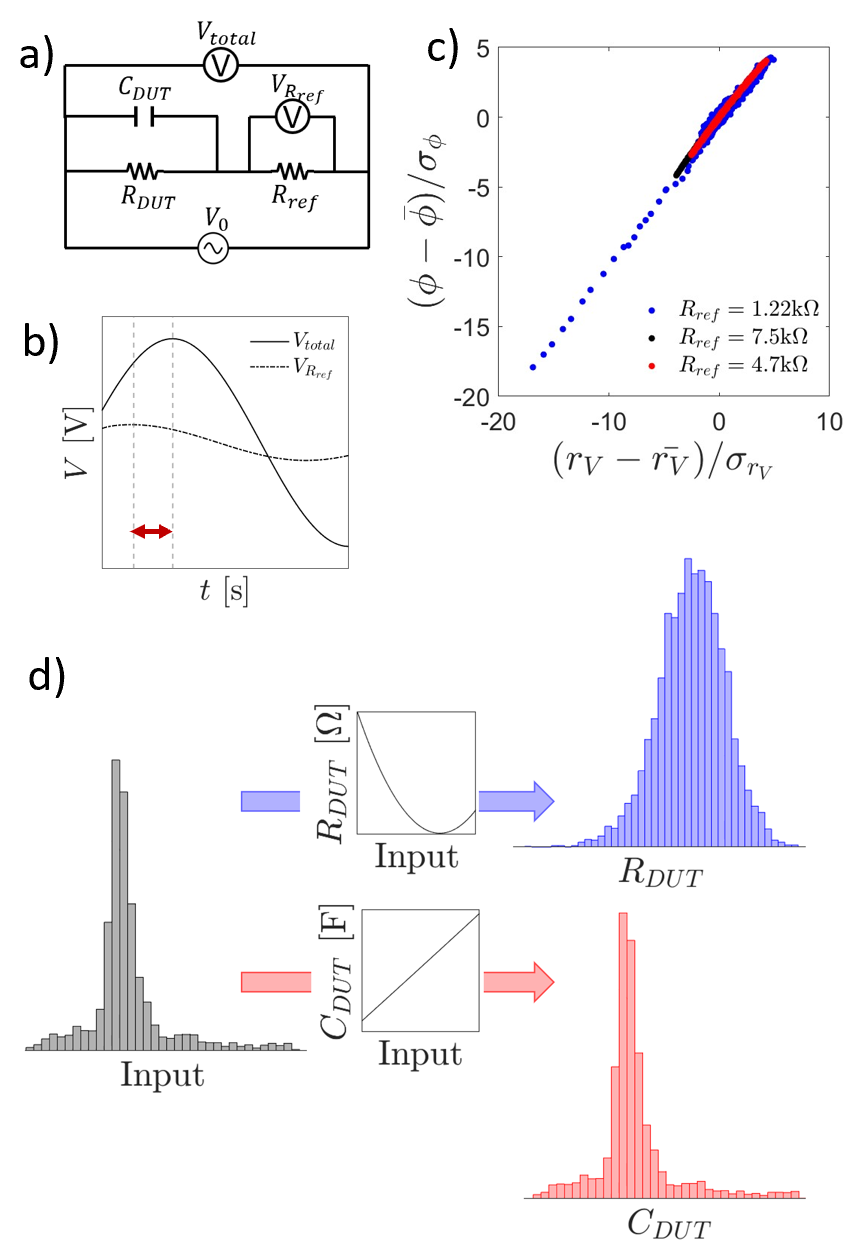
\includegraphics[width=0.45\textwidth]{./figures/basic.png}
    \caption{(a) A schematic of the experimental setup. $V_{\textrm{total}}$, $V_{R_{\textrm{ref}}}$ are both input probes to measure voltage, and a sinusoidal voltage source is given via $V_0$. $R_{\textrm{DUT}}$, $C_{\textrm{DUT}}$ are each the resistance and capacitance device under test, and $R_{\textrm{ref}}$ is the reference resistor. (b) Experimental values of $V_{\textrm{total}}$, $V_{R_{\textrm{ref}}}$. The red arrow depicts the measured phase difference($\phi$). (c) Scatter plot of normalized voltage ratio $(r_V-\bar{r_V})/\sigma_{r_V}$ and normalized phase difference $(\phi-\bar{\phi})/\sigma_{\phi}$. (d) Diagram showing the different distributions resulting from the same input distribution ($r_V$, $\phi$). The insets shows $R_{\textrm{DUT}}(r_V, \phi)$,  $C_{\textrm{DUT}}(r_V, \phi)$ at the vicinity of $\bar{r_V}$, $\bar{\phi}$. This is the histogram derived from $4.7k\Omega$ experimental data.}
    \label{fig:basic}
\end{figure}

\subsection{DUT Values Distribution}
When analyzing the $5000$ repetition sample of $1000$Hz for all three reference resistors, the voltage amplitude ratio ($r_V$) and the phase difference ($\phi$) showed a linear behavior. This is emphasized by normalizing each variable (Fig. \ref{fig:basic}(c)) 

The distributions for $R_{\textrm{DUT}}$ and $C_{\textrm{DUT}}$ calculated from the $5000$ repetition experiments are also shown in the colored insets of Fig. \ref{fig:basic}(d). The input distribution denotes $r_V$ (or $\phi$). The distribution of $C_{\textrm{DUT}}$ is nearly identical to the input distribution, while the distribution of $R_{\textrm{DUT}}$ has no clear relation. Note that every distribution analyzed rejected the Kolmogorov-Smirnov test for normality, i.e., none can be considered normal(Supplementary Information Section 1.).

The distribution of $R_{\textrm{DUT}}$ and $C_{\textrm{DUT}}$ are related to how input parameters ${r}_V$ and ${\phi}$ associate with $R_{\textrm{DUT}}, C_{\textrm{DUT}}$. The distribution of $C_{\textrm{DUT}}$ is similar to that of the input since the response of $C_{\textrm{DUT}}$ is linear to both ${r}_V$ and ${\phi}$. However, the distribution of $R_{\textrm{DUT}}$ differs due to the nonlinearity of $R_{\textrm{DUT}}$,  effectively 'folding' a portion of the input distribution. This tendency makes the distribution of $R_{\textrm{DUT}}$ thicker than that of the input. This observation allows us to expect how DUT parameters are distributed from the given input distribution and vice versa.


\begin{figure*}
    \centering
    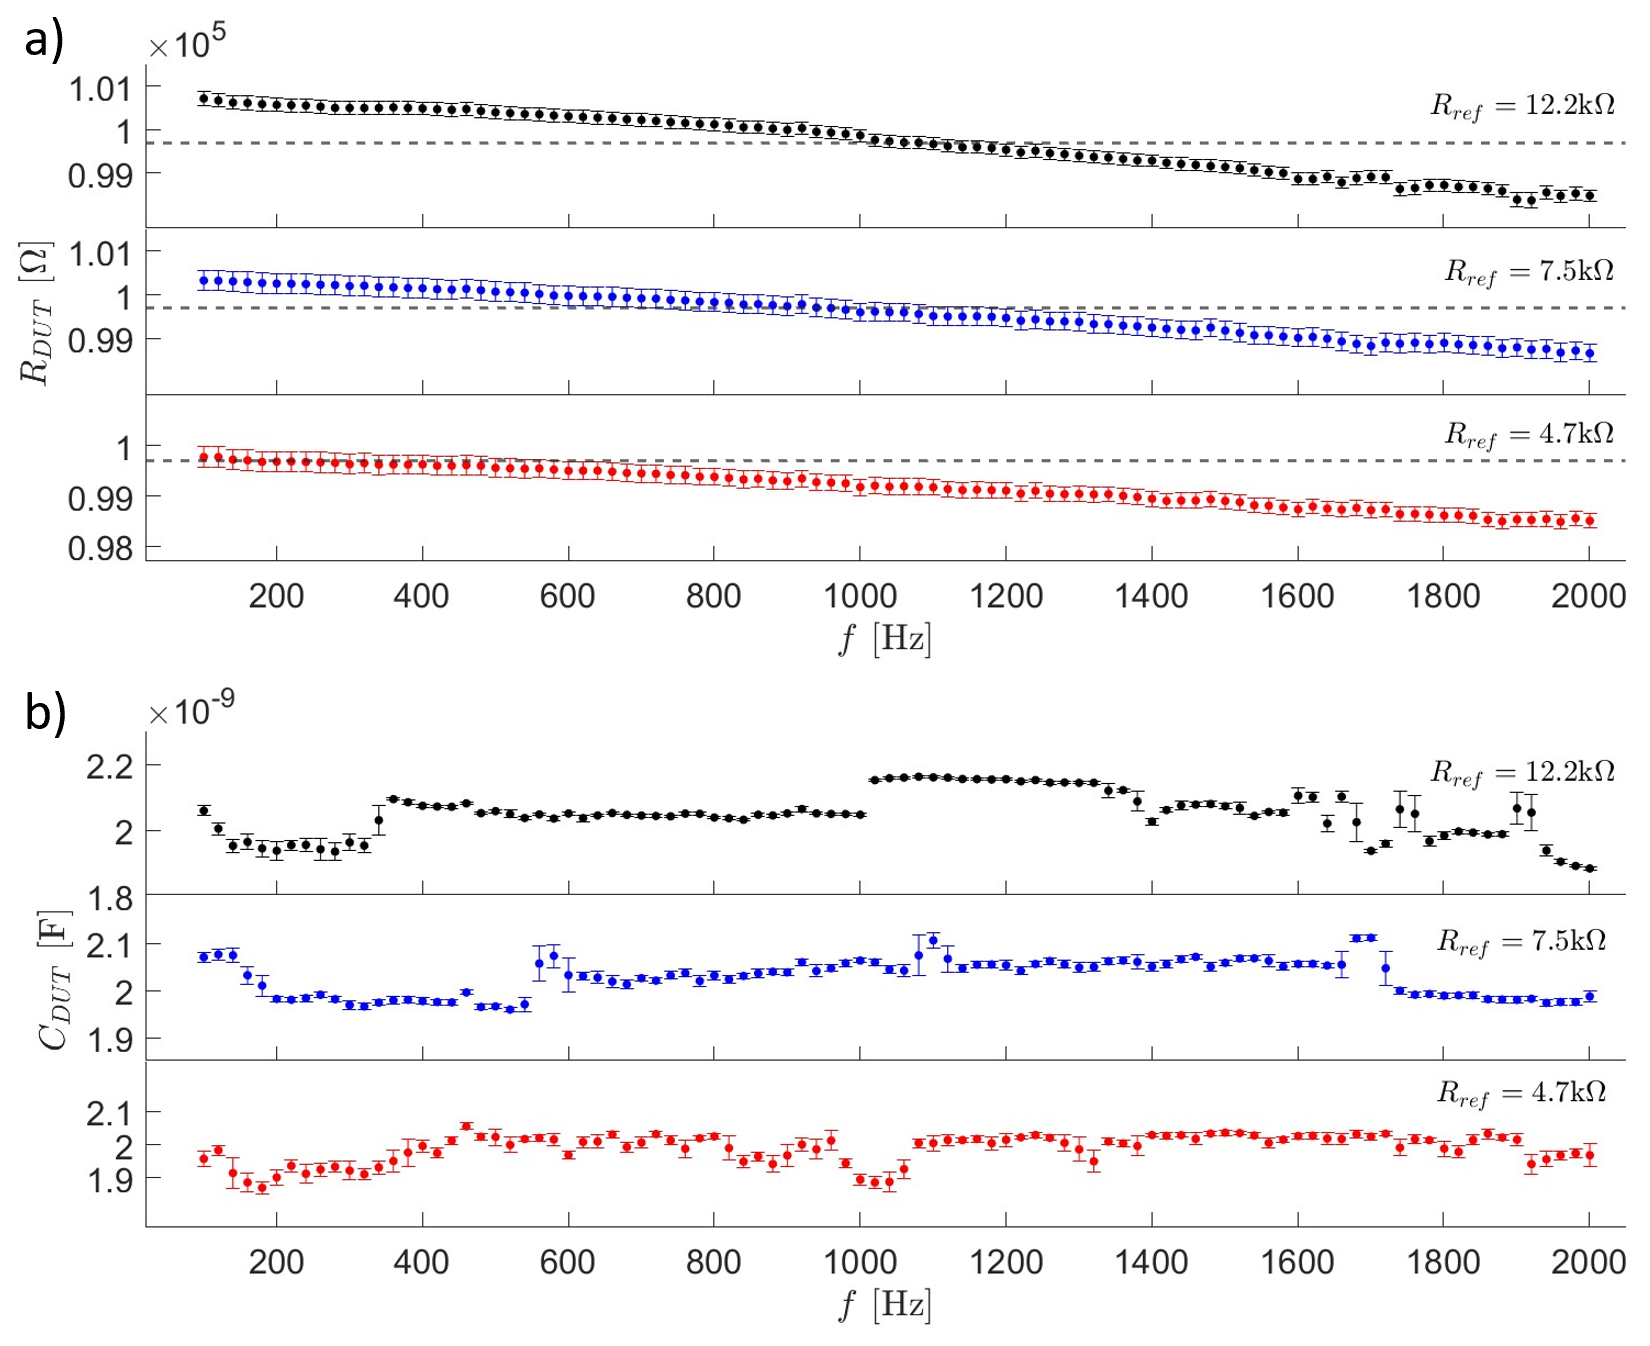
\includegraphics[width=0.9\textwidth]{./figures/dut total fig.png}
    \caption{Experimental (a) $R_{\textrm{DUT}}$ and (b) $C_{\textrm{DUT}}$ values by input AC voltage frequency. The error bars indicate the total error(statistical+systematic). Each color indicates a different reference resistor in use. The gray dashed line in (a) depicts the multimeter measured value $99.7\text{k}\Omega$ of $R_{\textrm{DUT}}$. Frequency error bars are smaller than the marker.}
\end{figure*}

\subsection{DUT Frequency Response}

The calculated $R_{\textrm{DUT}}$, $C_{\textrm{DUT}}$ values and the total error(statistical + systematic) at each frequency are shown in Fig. 2. The calculated $R_{\textrm{DUT}}$ values result near the multimeter measured $R_{\textrm{DUT}}$ value,  $99.7\pm0.15\text{k}\Omega$. In all reference resistors used, the experimental $R_{\textrm{DUT}}$ value shows a linear decrease over frequencies. Multiple effects have been considered to explain this linear decrease of $R_{\textrm{DUT}}$ at higher frequencies. 
 
 The control experiments remove the effects of the circuit other than the DUT, thus, these are discarded as a cause.

 Direct consideration of parasitic elements in the background circuit by calculating the background inductance from the negative linear relation (Supplementary Information Section 2.) between the phase difference and the system frequency in control experiments. The calculated background inductance was not constant about reference resistance. This is inconsistent with the assumption of a background inductance, also discarding circuit background inductance from a possible cause.

 The input impedance of the Analog Discovery 2 has been also considered. This however failed to resolve the problem, thus the input impedance is discarded from the possible cause.

All devices contain unexpected electric properties, called parasitic components\cite{parasite}. The parasitic capacitance of $R_{\textrm{DUT}}$ is combined with $C_{\textrm{DUT}}$, and thus is neglected. When considering the parasitic inductance ($L_{\textrm{p}}$) of each resistor, this resulted in a bigger $R_{\textrm{DUT}}$ at higher frequencies (Supplementary Information Section 3.). This is inconsistent with our experimental result, also discarding parasitic inductance as a possible cause.

\begin{comment}
    By assuming the parasitic inductance to be in series with the reference (or DUT) resistor, the obtained $R_{\textrm{DUT}}$ is a function of $L_{\textrm{p}}$. Since we performed the experiment in a low-frequency range, $L_{\textrm{p}}$ should be small enough to approximate to the first order. The coefficient of $L_{\textrm{p}}$ in first order was positive, resulting in a bigger $R_{\textrm{DUT}}$ at higher frequencies. This is inconsistent with our experimental result also discarding parasitic inductance from a possible cause.
\end{comment}



 The experimental $C_{\textrm{DUT}}$ values were smaller than the factory-listed capacitance $2.2$nF. Furthermore, compared to the experimental $R_{\textrm{DUT}}$ values, the $C_{\textrm{DUT}}$ values showed a higher degree of fluctuation, which are neither continuous nor uniform in trend among different reference resistances. Therefore, we believe such measurements are caused by real capacitance fluctuations, explained in detail at \textbf{\textit{\textsf{Statistical Error}}} in section \ref{sec:statisticalError}.



\begin{figure}
    \centering
    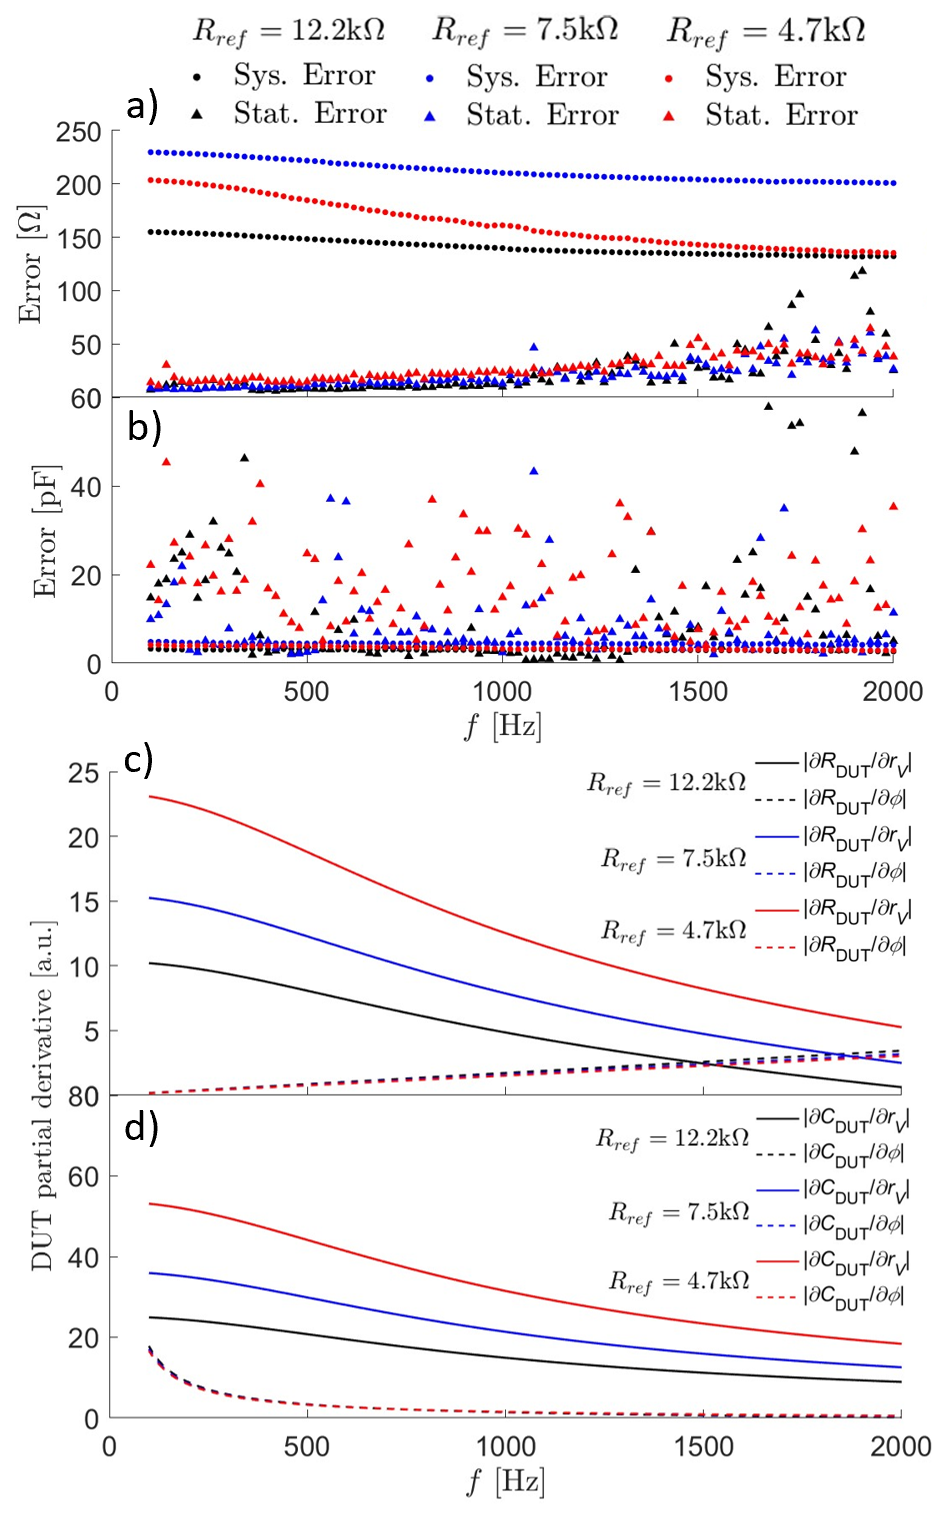
\includegraphics[width=0.45\textwidth]{./figures/errorandsensitivity.png}
    \caption{The (a) systematic and statistical error of $R_{\textrm{DUT}}$, (b) systematic and statistical error of $C_{\textrm{DUT}}$ by frequency. The calculated DUT $r_V$ and $\phi$ partial derivatives for (c) $R_{\textrm{DUT}}$ and (d) $C_{\textrm{DUT}}$. Each color indicates a different reference resistor in use.}
    \label{fig:error}
\end{figure}


\subsection{\label{sec:statisticalError}Error Effects on $R_{\textrm{DUT}}$, $C_{\textrm{DUT}}$ Measurements}
To analyze the frequency dependence of error, the error was divided into systematic and statistical errors. Each corresponding error for $R_{\textrm{DUT}}$, $C_{\textrm{DUT}}$ and the DUT derivatives $|\partial R_{\textrm{DUT}}/\partial r_V|$, $|\partial R_{\textrm{DUT}}/\partial \phi|$, $|\partial C_{\textrm{DUT}}/\partial r_V|$, $|\partial C_{\textrm{DUT}}/\partial \phi|$ were calculated (Fig. \ref{fig:error}). 

For the error of the $R_{\textrm{DUT}}$ measurements, the systematic error is larger than the statistical error. The systematic error also decreases as the frequency increases, much resembling the DUT derivative $|\partial R_{\textrm{DUT}}/\partial r_V|$  (Fig. \ref{fig:error} (a), (c)). The statistical error on the other hand increases with the frequency, resembling the DUT derivative $|\partial R_{\textrm{DUT}}/\partial \phi|$ (Fig. \ref{fig:error} (a), (c)). 

 We showed, by calculating the propagated systematic error of the DUT values, the systematic error indeed is considerable and can be minimized by selecting regions where the DUT partial derivative with respect to measured experimental quantities is minimized.
 
For the error of the $C_{\textrm{DUT}}$ measurements, the systematic error has a similar magnitude to the statistical error, and the statistical error shows extreme fluctuations throughout different frequencies. No typical resemblance can be observed with either DUT derivatives  $|\partial C_{\textrm{DUT}}/\partial r_V|$, $|\partial C_{\textrm{DUT}}/\partial \phi|$ (Fig. \ref{fig:error} (b), (d)).

 
\subsubsection*{Statistical Error}
The correlation between the voltage ratio and the phase difference strongly implies that there exists a significant factor which simultaneously changes the phase difference and voltage ratio. From Fig.\ref{fig:basic} (d), $C_{\textrm{DUT}}$ has a similar distribution with the phase difference and voltage ratio. We conjecture that the deviation of $\phi$ and $r_V$ possibly originated from the fluctuations of $C_\textrm{DUT}$.
\begin{comment}
    We conjectured that the fluctuation of the capacitor is bigger than other devices, so that the deviation of $\phi$ and $r_V$ depends almost only on  DUT capacitance. 
\end{comment}
Fig.\ref{fig:stdphiandRC} illustrates this tendency. According to Fig.\ref{fig:stdphiandRC}, the deviation of phase difference is linearly related to the capacitance of DUT, while resistance is well localized and randomly scattered. Also, the relative deviation of the DUT capacitance value is bigger than that of the resistance value. Furthermore, this resolves the fluctuations in the frequency response of the capacitor(Fig. 2(b)), and relatively high statistical error (Fig. \ref{fig:stdphiandRC}(b)). These results in unison support that the actual value of DUT capacitance fluctuations is relatively significant, and this is the main cause of the statistical error of this measurement.


\begin{figure}[!h]
    \centering
    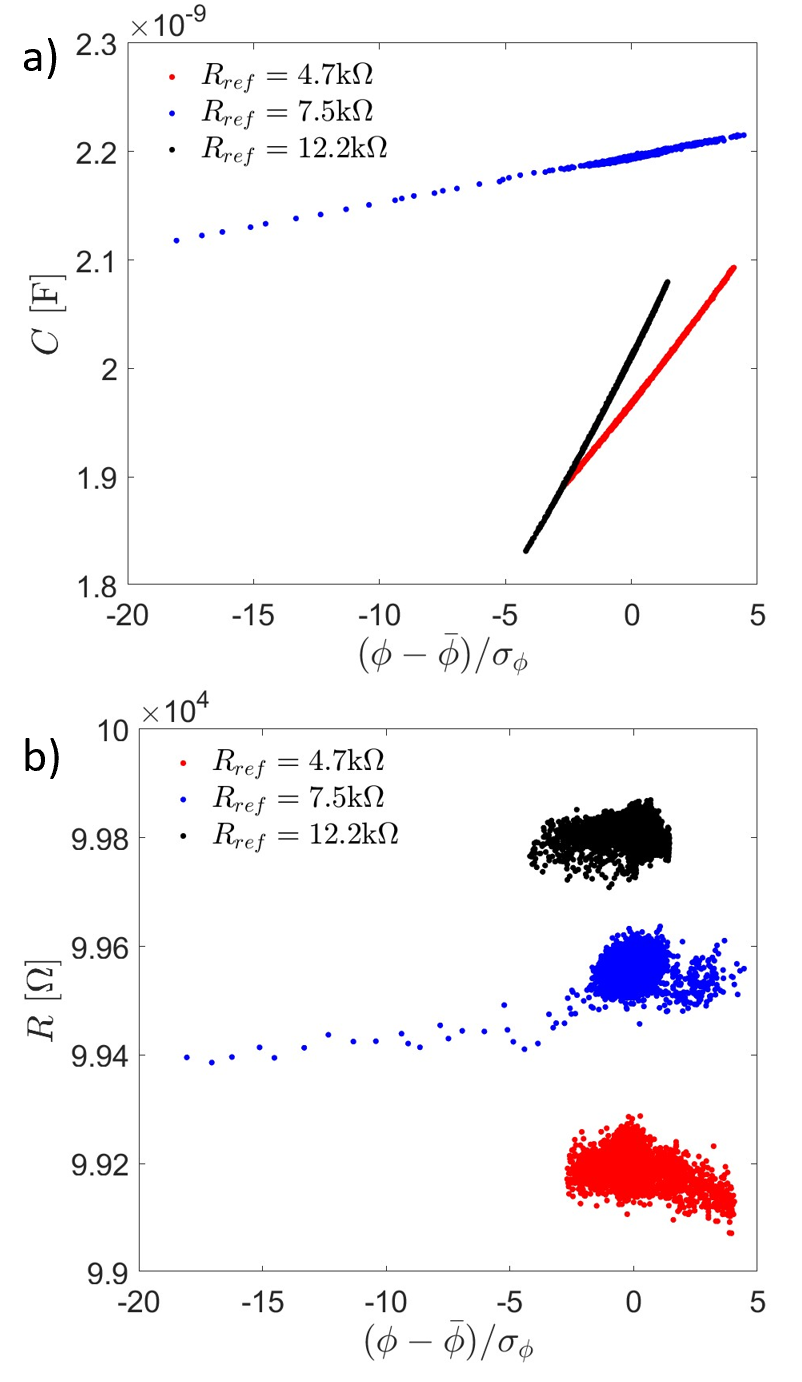
\includegraphics[width=0.45\textwidth]{./figures/stdphiandRC.png}
    \caption{The (a) capacitance and (b) resistance about the normalized deviation of phase difference. }
    \label{fig:stdphiandRC}
\end{figure}

\begin{comment}
    \subsection{DUT Frequency Response}
 Multiple effects have been considered to explain the linear decrease of $R_{\textrm{DUT}}$ at higher frequencies. 
 
 The control experiments remove the effects of the circuit other than the DUT, thus, these are discarded as a cause.

 Direct consideration of parasitic elements in the background circuit by calculating the background inductance from the negative linear relation between the phase difference and the system frequency in control experiments. The calculated background inductance was not constant about reference resistance. This is inconsistent with the assumption of a background inductance, also discarding circuit background inductance from a possible cause.
 
 The input impedance of the Analog Discovery 2 has been also considered. This however failed to resolve the problem, thus the input impedance is discarded from the possible cause.

All devices contain unexpected electric properties, called parasitic components\cite{parasite}. The parasitic capacitor component of $R_{\textrm{DUT}}$ is combined with $C_{\textrm{DUT}}$, and thus is neglected. When considering the parasitic inductance ($L_{\textrm{p}}$) of each resistor, this resulted in a bigger $R_{\textrm{DUT}}$ at higher frequencies. 

By assuming the parasitic inductance to be in series with the reference (or DUT) resistor, the obtained $R_{\textrm{DUT}}$ is a function of $L_{\textrm{p}}$. Since we performed the experiment in a low-frequency range, $L_{\textrm{p}}$ should be small enough to approximate to the first order. The coefficient of $L_{\textrm{p}}$ in first order was positive, resulting in a bigger $R_{\textrm{DUT}}$ at higher frequencies. This is inconsistent with our experimental result also discarding parasitic inductance from a possible cause.

\\
 The high fluctuation in the frequency response of $C_{\textrm{DUT}}$ is neither continuous nor uniform in trend among different reference resistances. Therefore, we believe such measurements are caused by real capacitance fluctuations, explained in detail at section \ref{sec:statisticalError}.
\end{comment}

\begin{comment}
    \subsection{Statistical Distributions of $R_{\textrm{DUT}}$, $C_{\textrm{DUT}}$}

 For a given input distribution, the distribution of $R_{\textrm{DUT}}$ and $C_{\textrm{DUT}}$ appear in different forms (Fig. \ref{fig:basic}(d)). This is related to how input parameters ${r}_V$ and ${\phi}$ associate with $R_{\textrm{DUT}}, C_{\textrm{DUT}}$. The distribution of $C_{\textrm{DUT}}$ is similar to that of the input since the response of $C_{\textrm{DUT}}$ is linear to both ${r}_V$ and ${\phi}$. However, the distribution of $R_{\textrm{DUT}}$ differs due to the nonlinearity of $R_{\textrm{DUT}}$,  effectively 'folding' a portion of the input distribution. This tendency makes the distribution of $R_{\textrm{DUT}}$ thicker than that of the input. This observation allows us to expect how DUT parameters are distributed from the given input distribution and vice versa.
\end{comment}


\begin{comment}
\begin{acknowledgments}
We wish to acknowledge the support of the author community in using
REV\TeX{}, offering suggestions and encouragement, testing new versions,
\dots.
\end{acknowledgments}
    
\end{comment}

\section{Conclusion}

In conclusion, we measured $R_{\textrm{DUT}}$ and $C_{\textrm{DUT}}$ using an AC voltage input. For three reference resistors, single frequency experiments and frequency sweeps were analyzed to measure DUT value distributions and the frequency dependence, including error analysis with statistical methods and systematic error propagation. 

Results showed accurate values of DUT components and correlations between DUT partial derivatives and systematic error. A high correlation between the distributions of $C_{\textrm{DUT}}$, $r_V$, and $\phi$ have been observed. An intrinsic fluctuation of the capacitor component is conjectured to be a major cause of the measured fluctuation of the DUT capacitance, also being the origin of the voltage ratio and phase difference distribution correlation. Such fluctuation could be analyzed further using repeated discharge measurements over a long time period.

In total, for measurement experiments using resistors and capacitors, (i) minimizing the DUT partial derivatives with respect to measured variables and (ii) prioritizing in stable capacitance more than resistance can substantially enhance the precision.

The cause of a decrease in DUT resistance about frequency is unresolved, however, we were able to discard (i) parasitic background circuit effects, (ii) parasitic inductance effects, and (iii) AD2 input impedance effects from the causes. This indicates that more complex physical phenomena of passive components, or the AD2 measurement device could be the cause. Further experimentation suitable for a wider range of frequencies would elucidate the cause.

\section*{Data Availability Statement}

The data that support the findings of this study are available from the corresponding author upon reasonable request.



\appendix

\section{Derivation of DUT values and their derivatives}

This section introduces derivations of theoretical DUT values and their derivatives which are mentioned at the beginning of the article. The impedance of the total circuit (Fig. 1(a)) is
\begin{align*}
Z&=R_{\textrm{ref}}+\frac{1}{\frac{1}{R_{\textrm{DUT}}}+i\omega C_{\textrm{DUT}}}\\
&=R_{\textrm{ref}}+\frac{R_{\textrm{DUT}}}{1+i\omega C_{\textrm{DUT}}R_{\textrm{DUT}}}\\
&=\frac{(R_{\textrm{ref}}+R_{\textrm{DUT}})+i\omega R_{\textrm{ref}} C_{\textrm{DUT}}R_{\textrm{DUT}}}{1+i\omega C_{\textrm{DUT}}R_{\textrm{DUT}}}
\end{align*}

\noindent The amplitude ratio($r_V$) is then,

\begin{equation*}
r_{V}=\frac{R_{\textrm{ref}}}{|Z|}=R_{\textrm{ref}}\sqrt{\frac{1+\omega^{2}C_{\textrm{DUT}}^{2}R_{\textrm{DUT}}^{2}}{(R_{\textrm{ref}}+R_{\textrm{DUT}})^{2}+\omega^{2}R_{\textrm{ref}}^{2}C_{\textrm{DUT}}^{2}R_{\textrm{DUT}}^{2}}}
\end{equation*}

\noindent Tangent of phase difference($\phi$) between the total voltage and the reference resistor is the ratio of the imaginary part and the real part of the impedance.

\begin{align*}
\tan\phi&=\frac{\textrm{Im}(Z)}{\textrm{Re}(Z)}\\
&=\frac{\omega R_{\textrm{ref}} C_{\textrm{DUT}}R_{\textrm{DUT}}-(R_{\textrm{ref}}+R_{\textrm{DUT}})\omega C_{\textrm{DUT}}R_{\textrm{DUT}}}{(R_{\textrm{ref}}+R_{\textrm{DUT}})+(\omega R_{\textrm{ref}} C_{\textrm{DUT}}R_{\textrm{DUT}})(\omega C_{\textrm{DUT}}R_{\textrm{DUT}})}\\
&=\frac{-\omega C_{\textrm{DUT}}R_{\textrm{DUT}}^{2}}{R_{\textrm{ref}}+R_{\textrm{DUT}}+\omega^{2} R_{\textrm{ref}}C_{\textrm{DUT}}^{2}R_{\textrm{DUT}}^{2}}
\end{align*}

\noindent To solve $r_{V}$ and $\phi$ for $R_{\textrm{DUT}}$ and $C_{\textrm{DUT}}$, we used vpasolve function given by MATLAB, constraining that $R_{\textrm{DUT}}\sim O(10^{5})$ and $C_{\textrm{DUT}}\sim O(10^{-9})$.

For derivatives, first note that

\begin{align}
&dr_{V}=\frac{\partial r_{V}}{\partial R_{\textrm{DUT}}}dR_{\textrm{DUT}}+\frac{\partial r_{V}}{\partial C_{\textrm{DUT}}}dC_{\textrm{DUT}}+\frac{\partial r_{V}}{\partial R_{\textrm{ref}}}dR_{\textrm{ref}}+\frac{\partial r_{V}}{\partial \omega}d\omega\\
&d\phi=\frac{\partial \phi}{\partial R_{\textrm{DUT}}}dR_{\textrm{DUT}}+\frac{\partial \phi}{\partial C_{\textrm{DUT}}}dC_{\textrm{DUT}}+\frac{\partial \phi}{\partial R_{\textrm{ref}}}dR_{\textrm{ref}}+\frac{\partial \phi}{\partial \omega}d\omega
\end{align}

\begin{align}
&dR_{\textrm{DUT}}=\frac{\partial R_{\textrm{DUT}}}{\partial r_{V}}dr_{V}+\frac{\partial R_{\textrm{DUT}}}{\partial \phi}d\phi+\frac{\partial R_{\textrm{DUT}}}{\partial R_{\textrm{ref}}}dR_{\textrm{ref}}+\frac{\partial R_{\textrm{DUT}}}{\partial \omega}d\omega\label{eq:rdut}\\
&dC_{\textrm{DUT}}=\frac{\partial C_{\textrm{DUT}}}{\partial r_{V}}dr_{V}+\frac{\partial C_{\textrm{DUT}}}{\partial \phi}d\phi+\frac{\partial C_{\textrm{DUT}}}{\partial R_{\textrm{ref}}}dR_{\textrm{ref}}+\frac{\partial C_{\textrm{DUT}}}{\partial \omega}d\omega
\label{eq:cdut}
\end{align}

\noindent We need to combine (A1) and (A2) and then arrange in the form of (A3) and (A4) in order to get derivatives. By doing so, we obtain the desired partial derivatives.
\begin{align}
&\frac{\partial R_{\textrm{DUT}}}{\partial r_{V}}=-\frac{\frac{\partial \phi}{\partial C_{\textrm{DUT}}}}{\frac{\partial \phi}{\partial R_{\textrm{DUT}}}\frac{\partial r_{V}}{\partial C_{\textrm{DUT}}} - \frac{\partial r_{V}}{\partial R_{\textrm{DUT}}}\frac{\partial \phi}{\partial C_{\textrm{DUT}}}}\\
&\frac{\partial R_{\textrm{DUT}}}{\partial \phi}=\frac{\frac{\partial r_{V}}{\partial C_{\textrm{DUT}}}}{\frac{\partial \phi}{\partial R_{\textrm{DUT}}}\frac{\partial r_{V}}{\partial C_{\textrm{DUT}}} - \frac{\partial r_{V}}{\partial R_{\textrm{DUT}}}\frac{\partial \phi}{\partial C_{\textrm{DUT}}}}
\end{align}

\begin{align}
&\frac{\partial C_{\textrm{DUT}}}{\partial r_{V}}=\frac{\frac{\partial \phi}{\partial R_{\textrm{DUT}}}}{\frac{\partial \phi}{\partial R_{\textrm{DUT}}}\frac{\partial r_{V}}{\partial C_{\textrm{DUT}}} - \frac{\partial r_{V}}{\partial R_{\textrm{DUT}}}\frac{\partial \phi}{\partial C_{\textrm{DUT}}}}\\
&\frac{\partial C_{\textrm{DUT}}}{\partial \phi}=-\frac{\frac{\partial r_{V}}{\partial R_{\textrm{DUT}}}}{\frac{\partial \phi}{\partial R_{\textrm{DUT}}}\frac{\partial r_{V}}{\partial C_{\textrm{DUT}}} - \frac{\partial r_{V}}{\partial R_{\textrm{DUT}}}\frac{\partial \phi}{\partial C_{\textrm{DUT}}}}
\end{align}


\bibliographystyle{unsrt}
\bibliography{./references/module1_bibtex}


\end{document}
%
% ****** End of file aipsamp.tex ******C